\documentclass[12pt,letterpaper]{article}

\usepackage{amsmath, amsthm}
\usepackage{microtype, parskip}
\usepackage[comma,numbers,sort&compress]{natbib}
\usepackage{lineno}
\usepackage{docmute}
\usepackage{caption, subcaption, multirow, morefloats, rotating}
\usepackage{wrapfig}

\frenchspacing

\captionsetup[subfigure]{position = top, labelfont = bf, textfont = normalfont, singlelinecheck = off, justification = raggedright}

\begin{document}
\section{Results}

% model fit
\begin{figure}[ht]
  \centering
  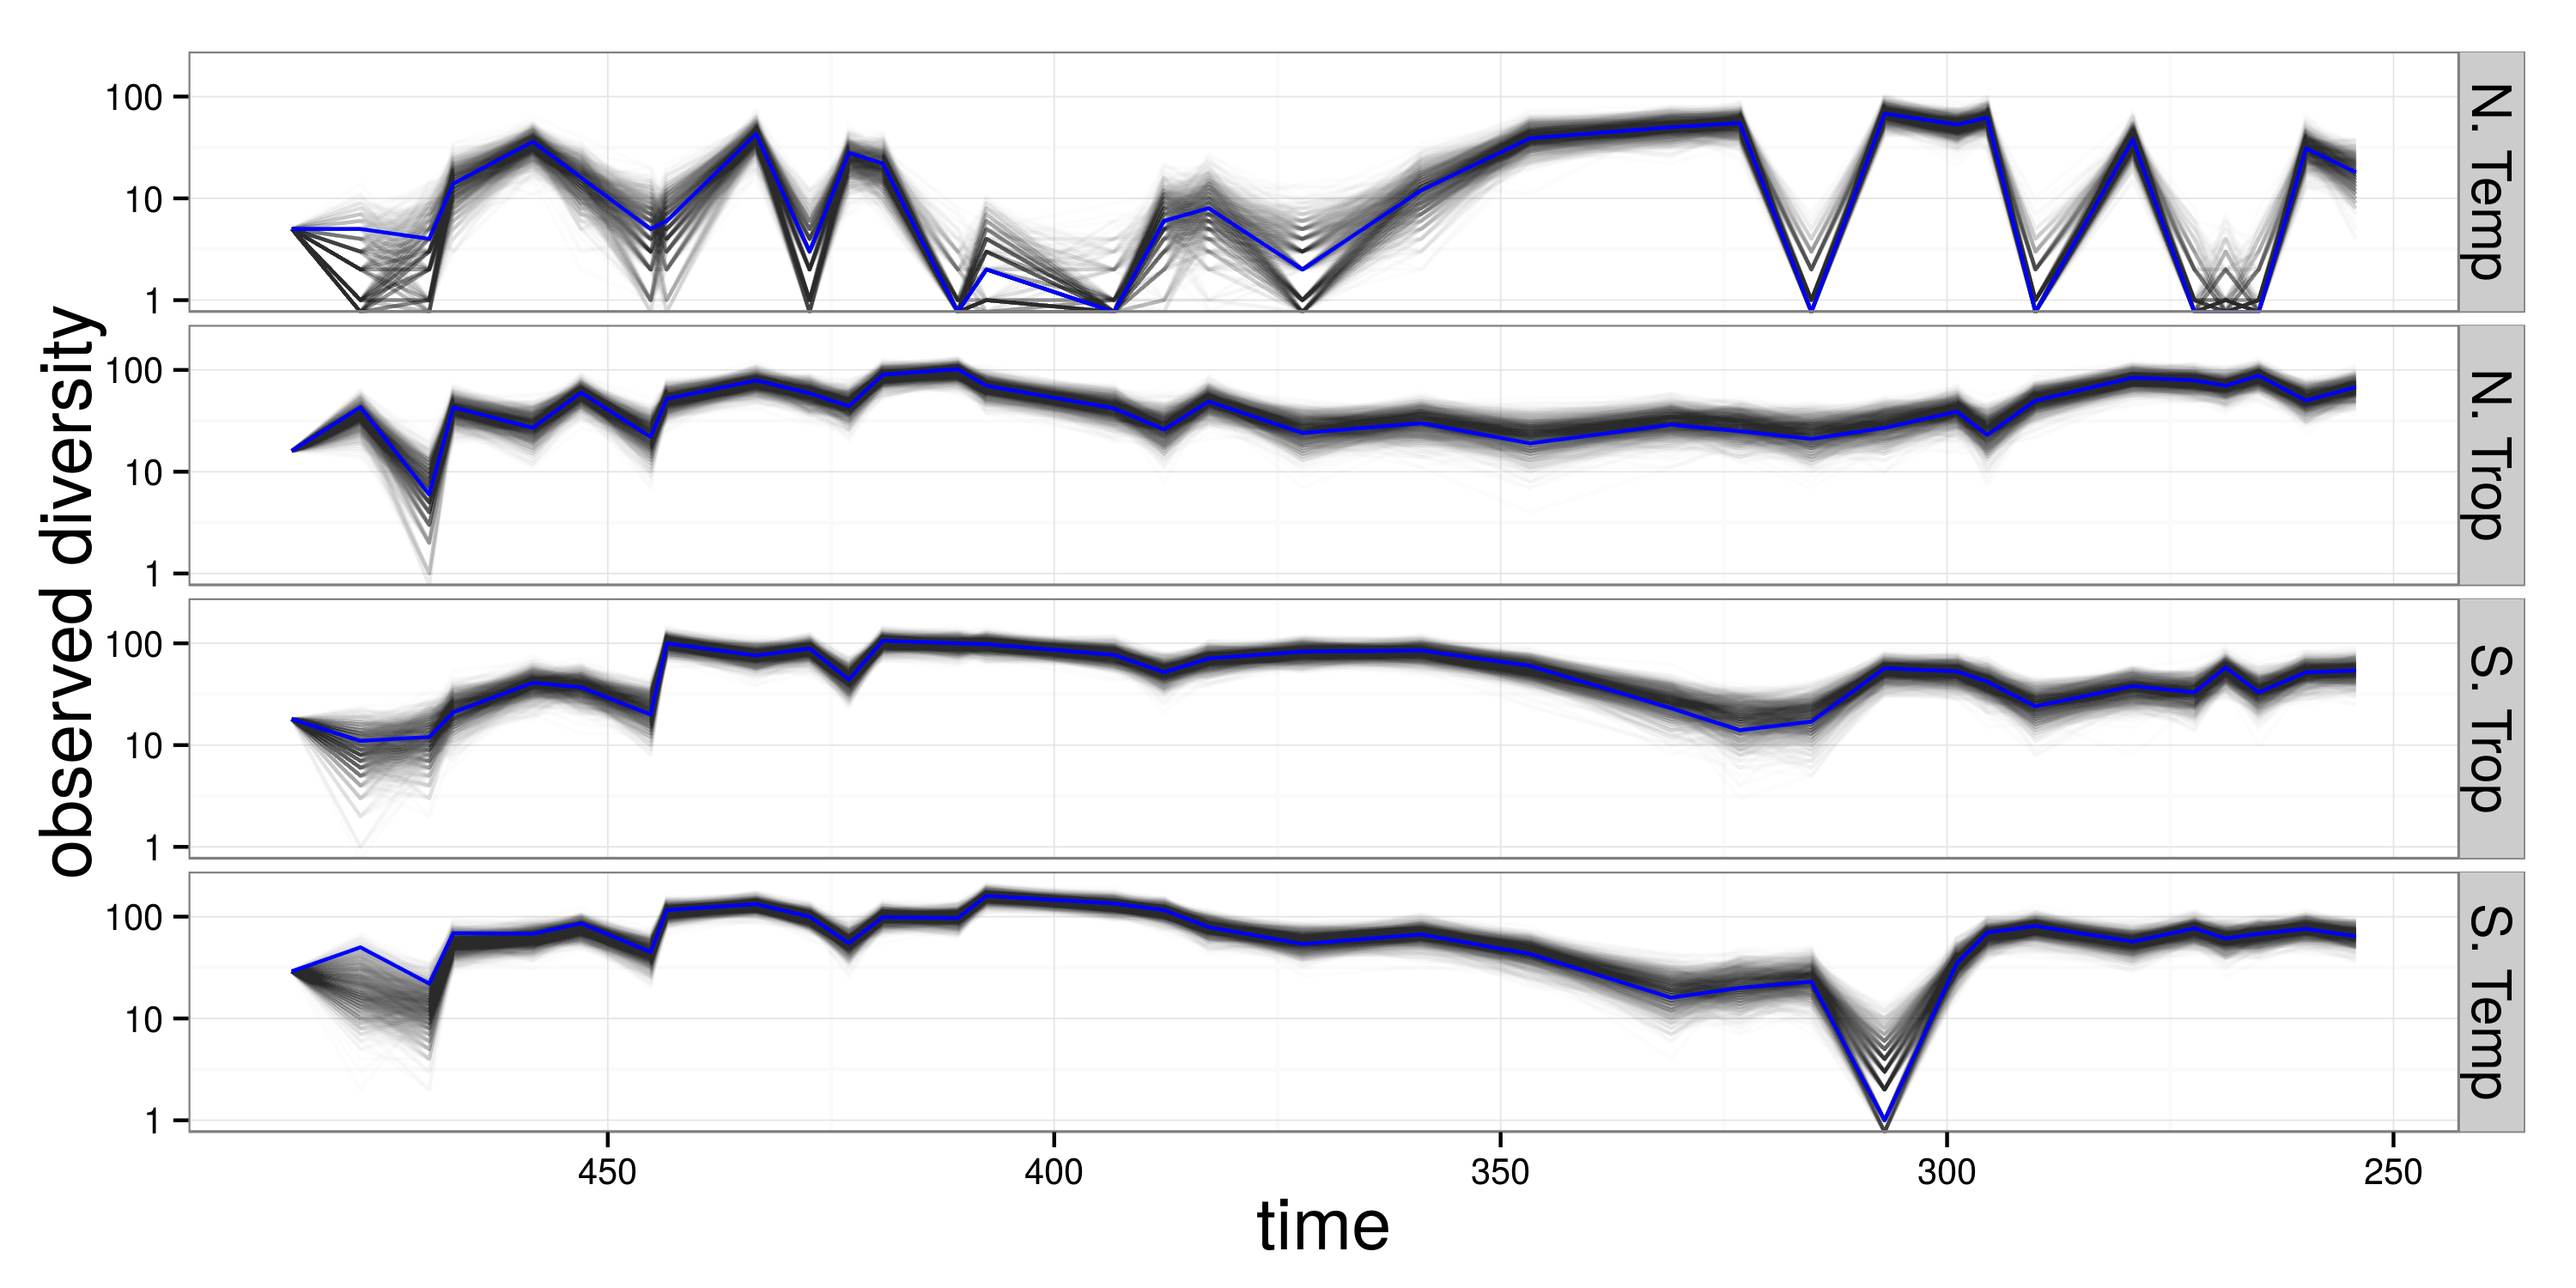
\includegraphics[width=\textwidth,height=0.5\textheight,keepaspectratio=true]{figure/obs_div}
  \caption{CAPTION}
  \label{fig:fit}
\end{figure}

% estimated ``true'' diversity
\begin{figure}[ht]
  \centering
  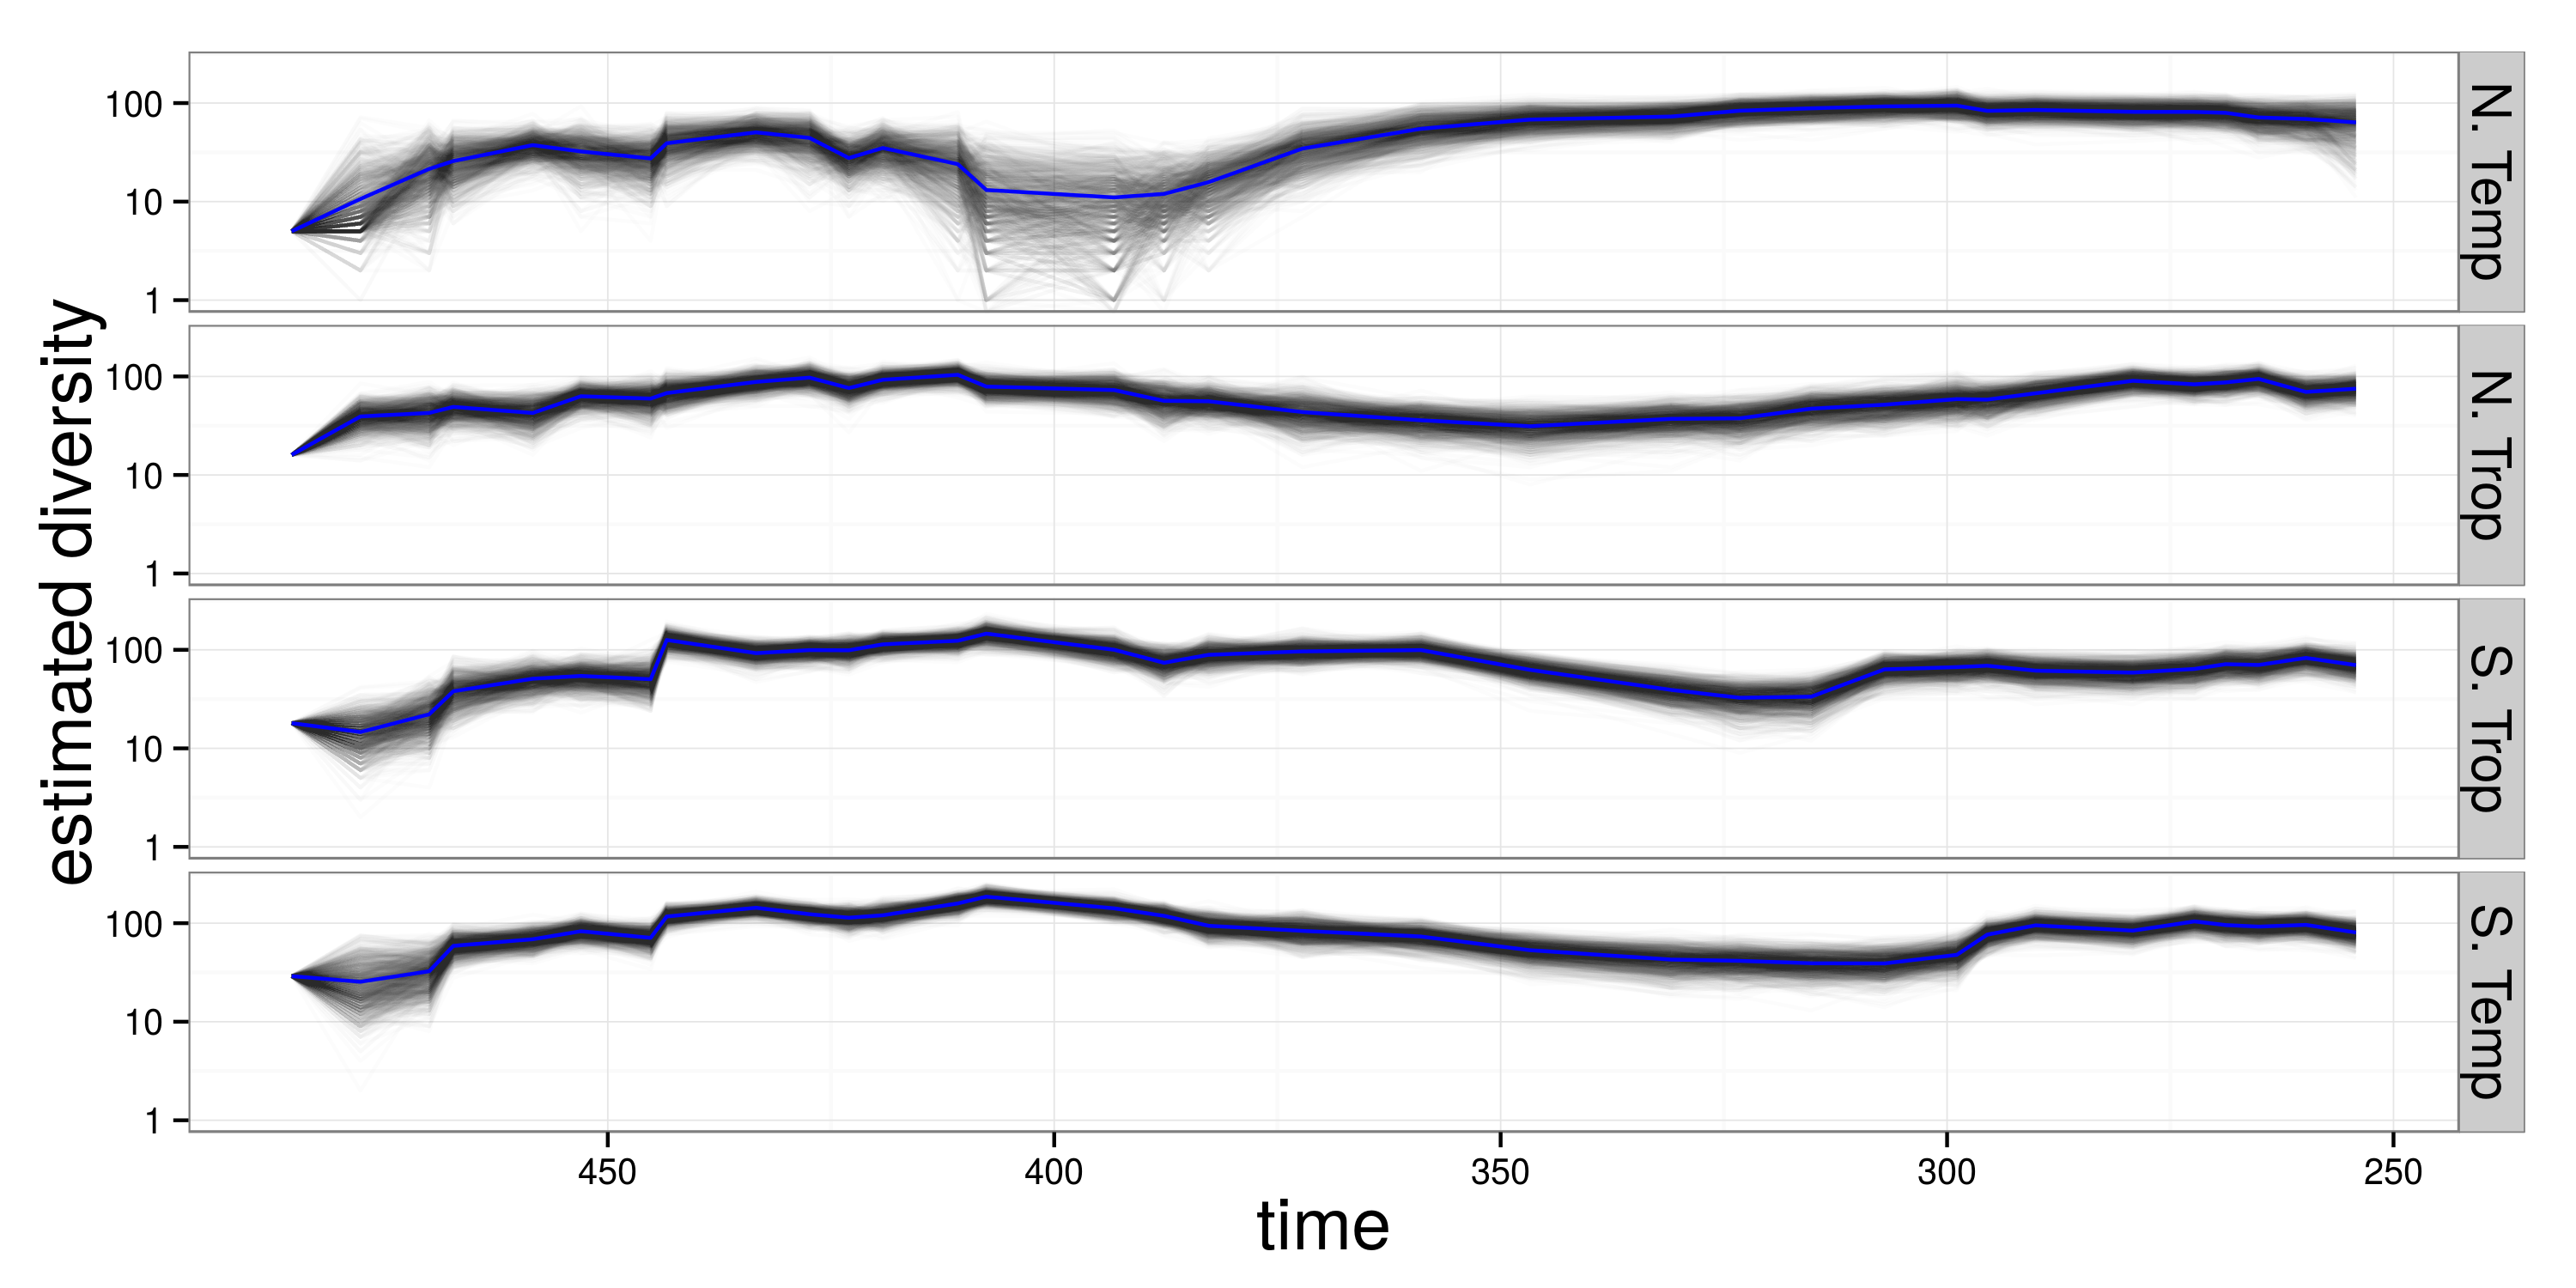
\includegraphics[width=\textwidth,height=0.5\textheight,keepaspectratio=true]{figure/true_div}
  \caption{CAPTION}
  \label{fig:true}
\end{figure}

% relative form
\begin{figure}[ht]
  \centering
  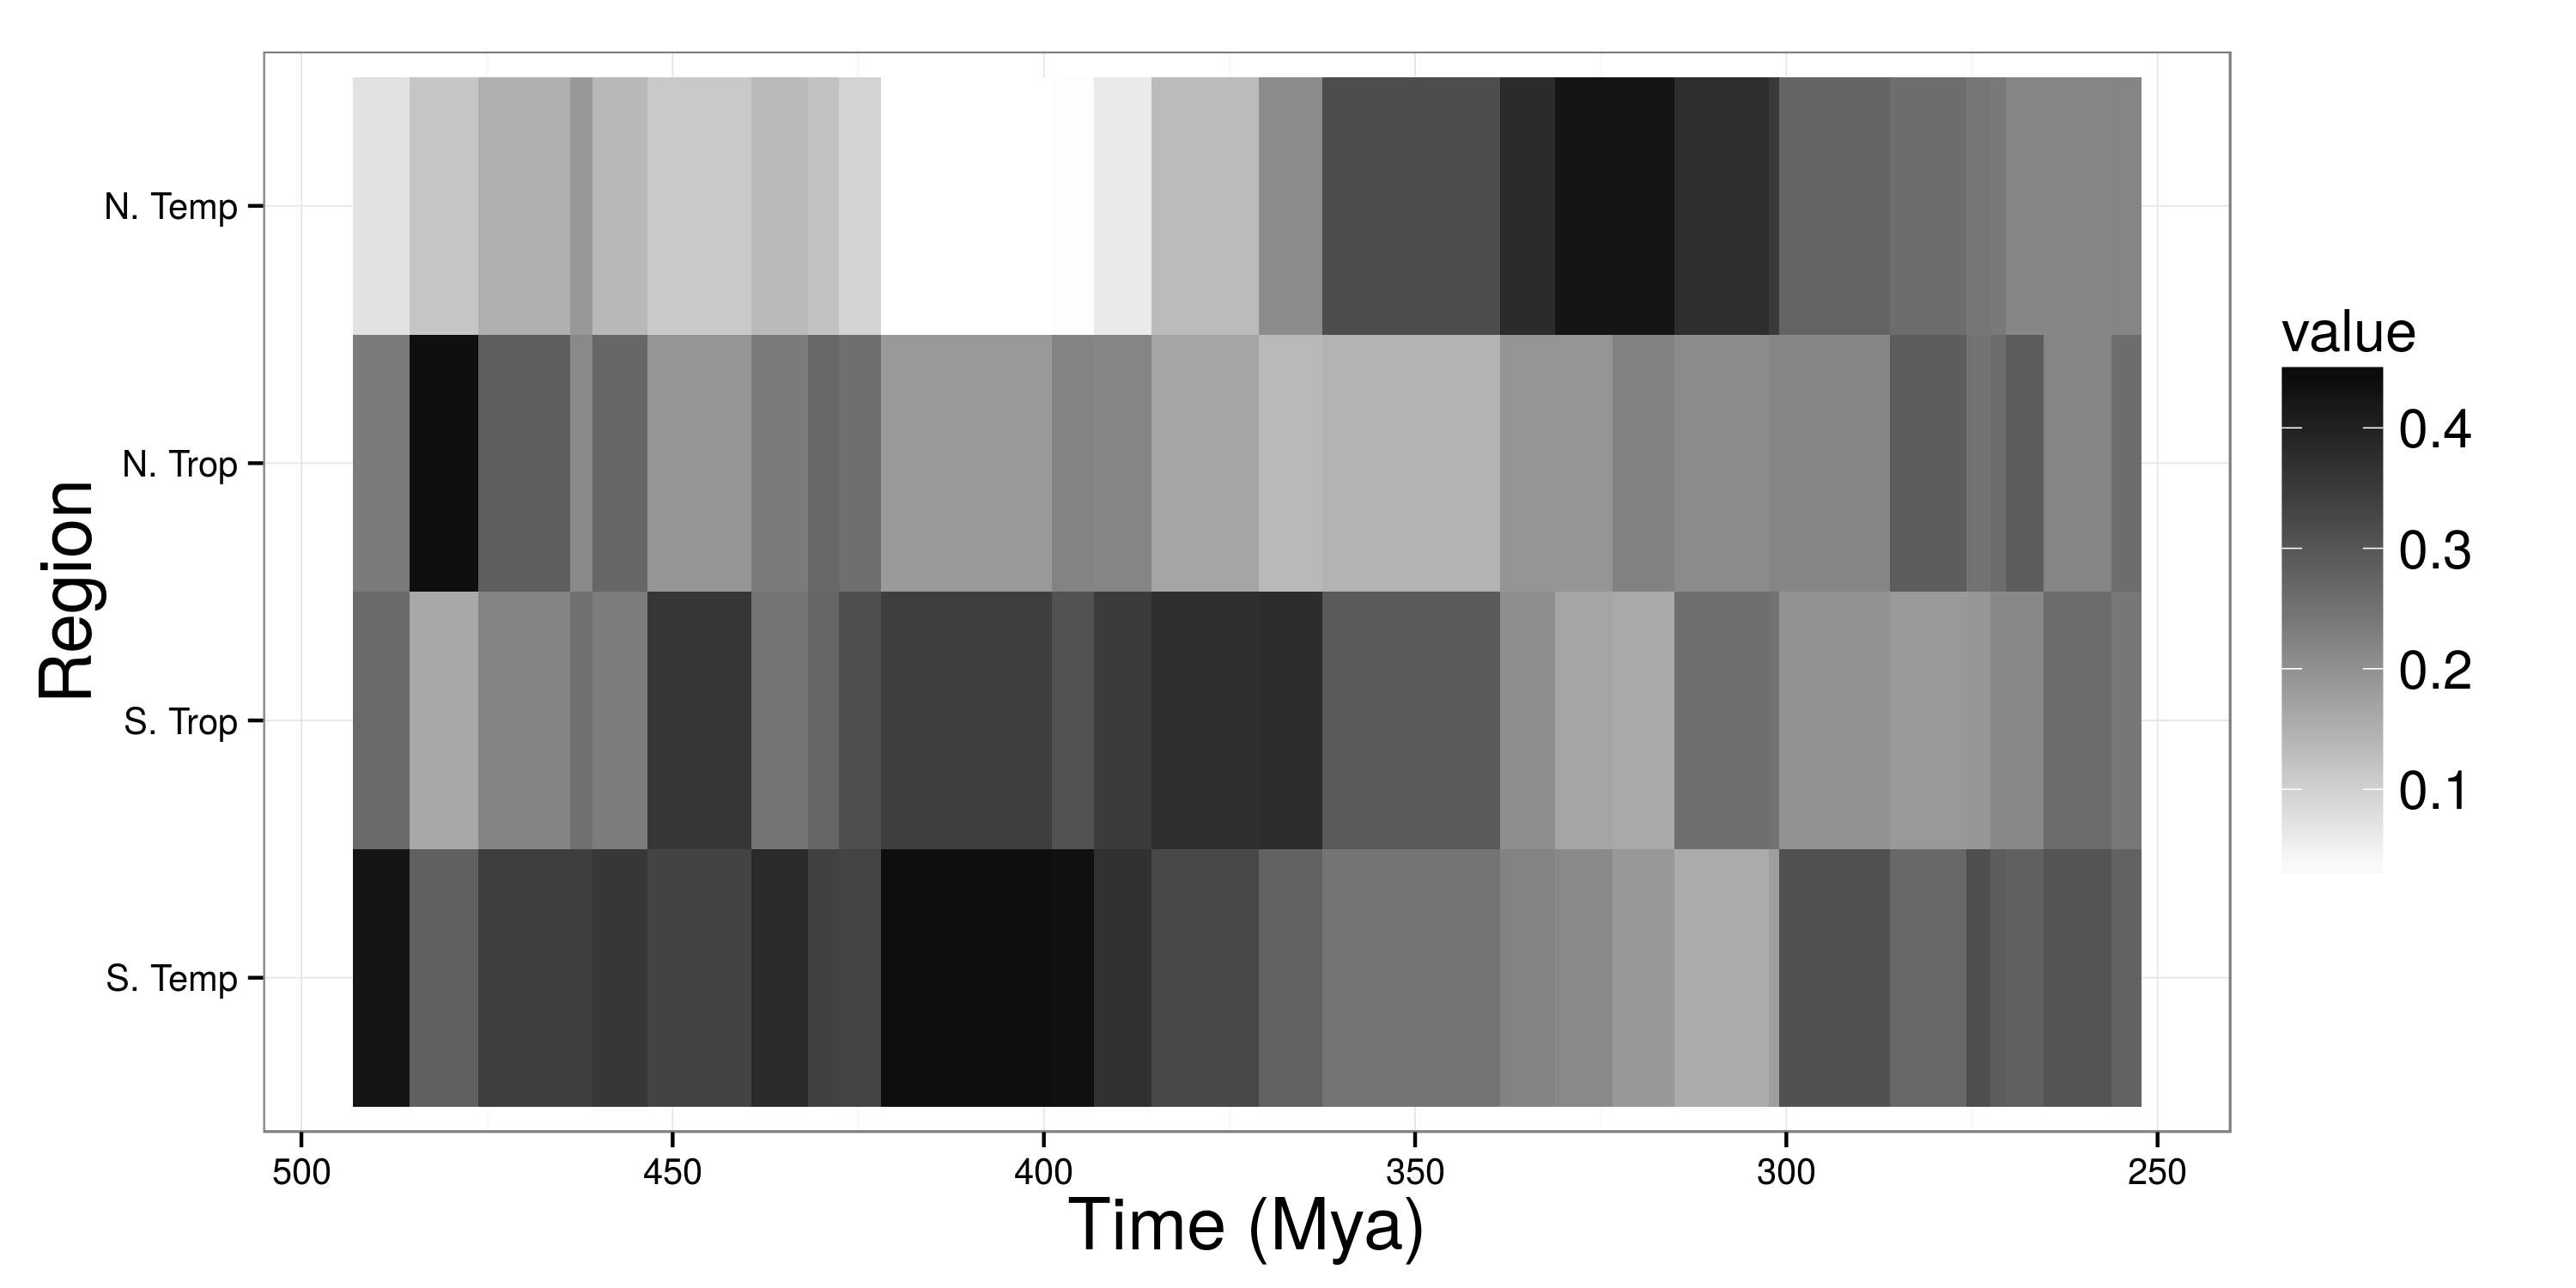
\includegraphics[width=\textwidth,height=0.5\textheight,keepaspectratio=true]{figure/rel_div}
  \caption{CAPTION}
  \label{fig:rel}
\end{figure}

% origination/entrance probability (or rate)
% extinction/loss probability (or rate)

% turnover (sense Royle and Dozario)
\begin{figure}[ht]
  \centering
  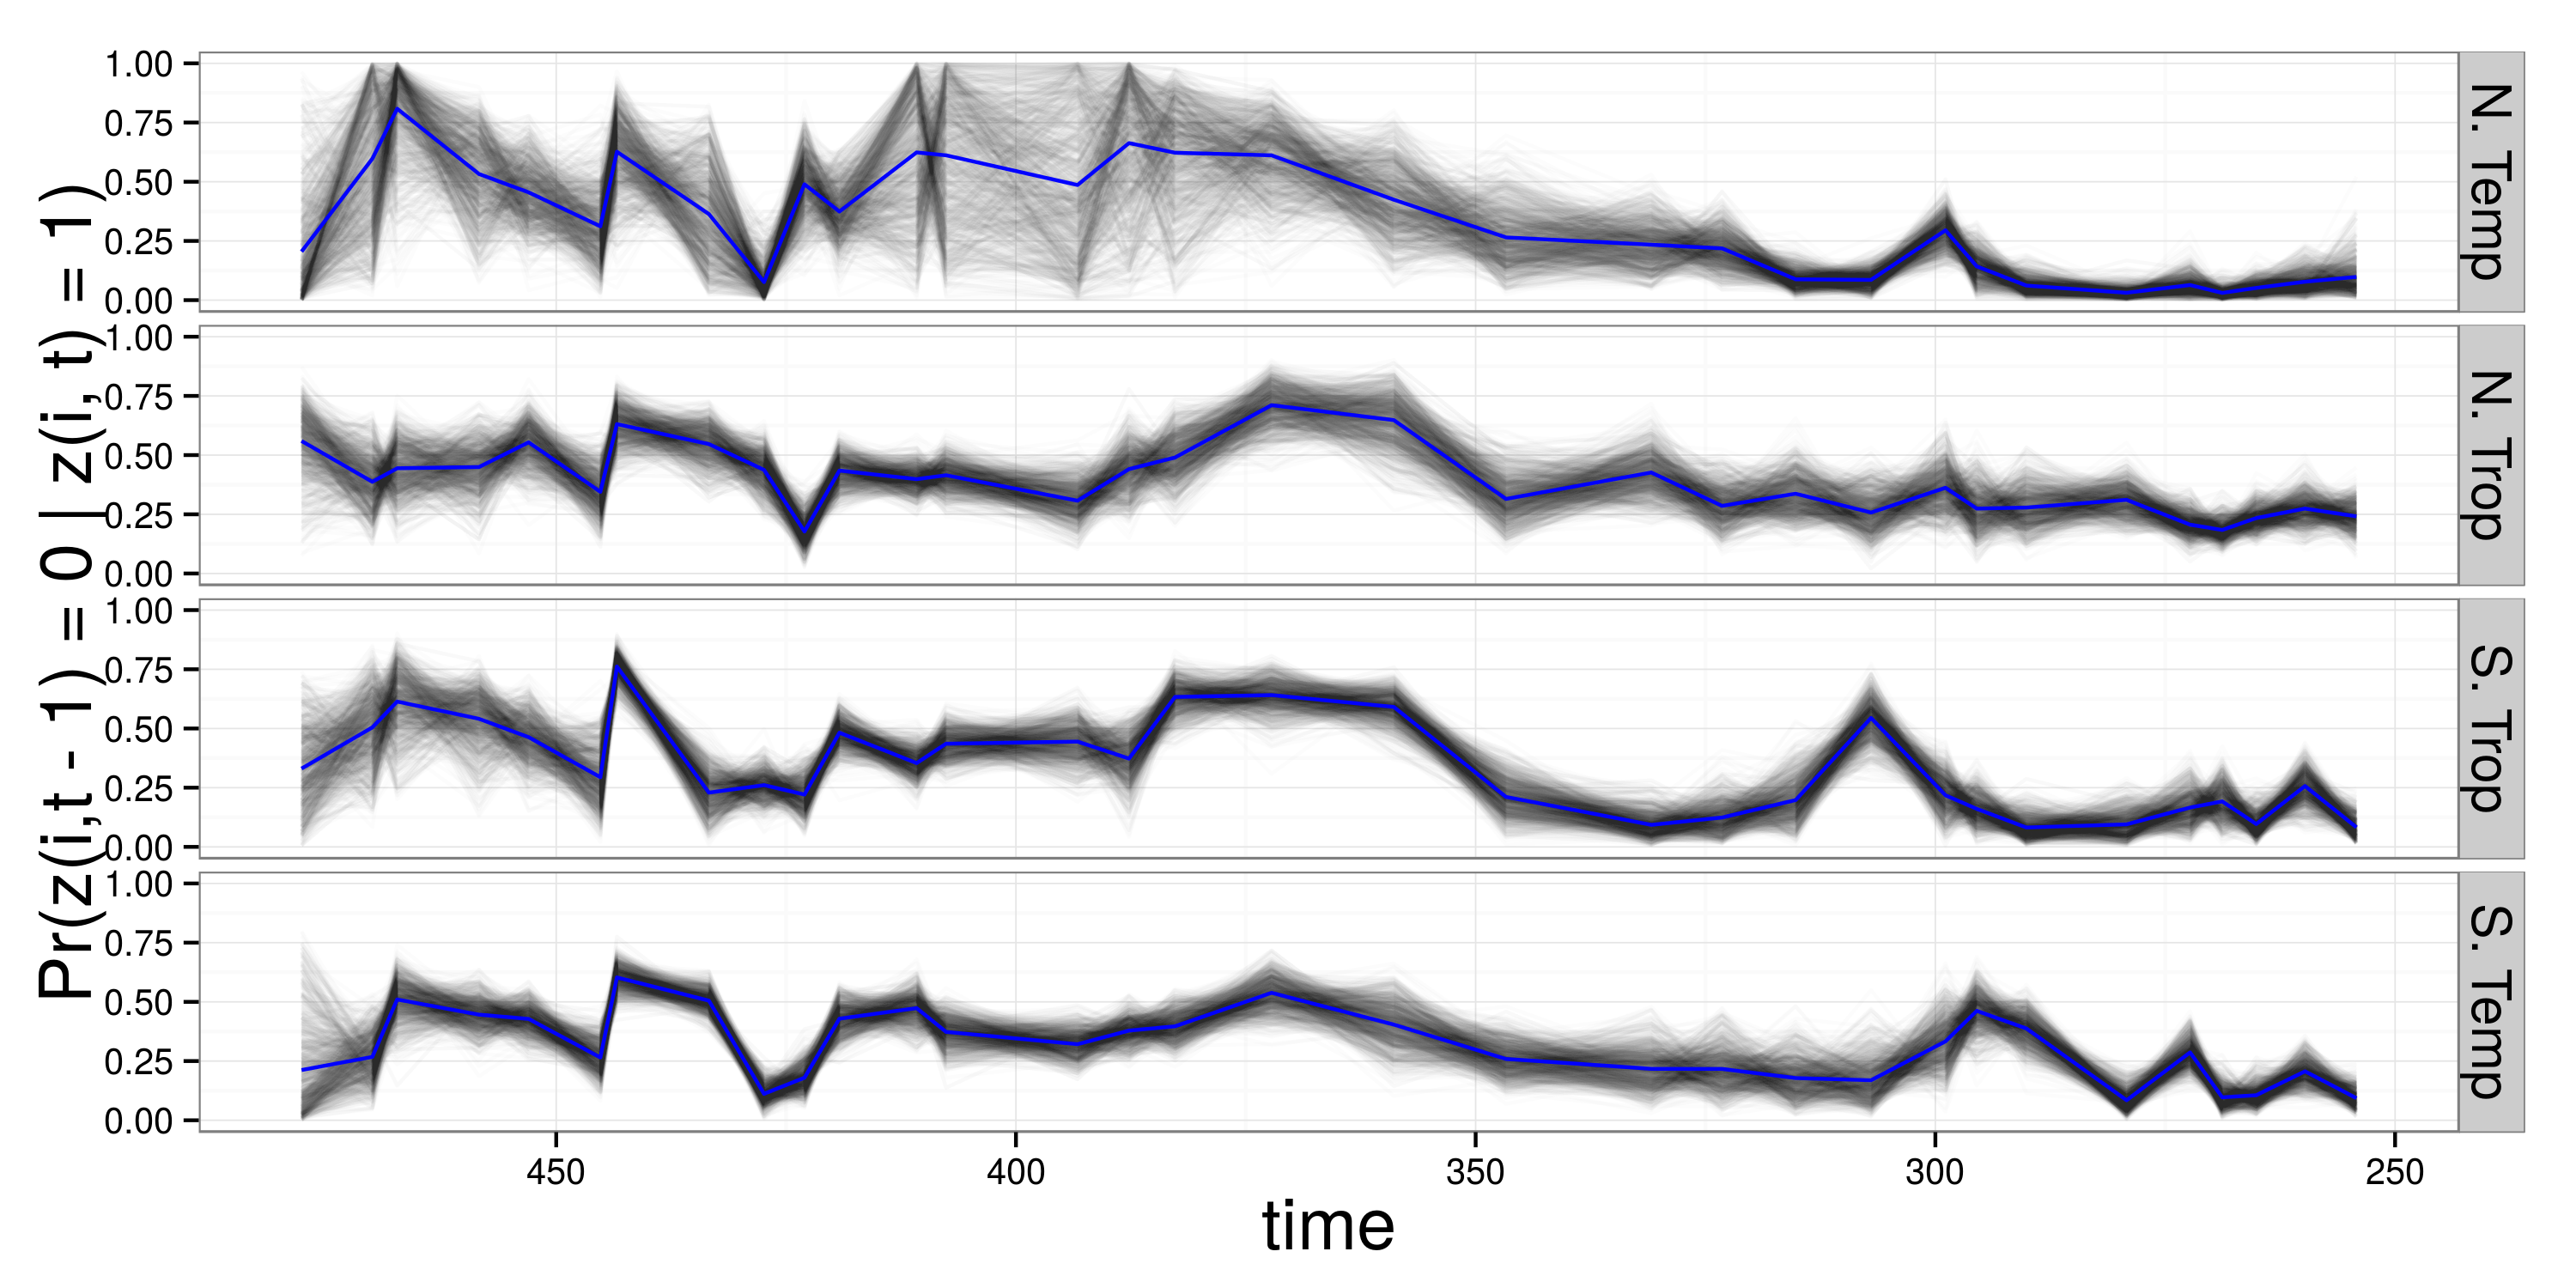
\includegraphics[width=\textwidth,height=0.5\textheight,keepaspectratio=true]{figure/turnover}
  \caption{CAPTION}
  \label{fig:turn}
\end{figure}

% what other derived statistics are there?

\end{document}
